The dominant source of prompt background in this analysis comes from $WZ$ events where both bosons decay leptonically.
Traditionally, the background is dealt with by imposing a veto on any event with a third lepton passing some loose identification criteria (the so-called \emph{trilepton veto}).
In the case of this analysis, if one or more leptons (in addition to the two signal leptons) passed the preselection criteria, the event would be rejected.
However, $WZ$ events can still enter the signal region if one of the leptons fails the veto selection or falls outside of the detector's acceptance.

In order to understand the sources of $WZ$ events that are not removed by the trilepton veto, a study was performed on truth-level leptons\footnote{Truth particles are the particles produced directly by the MC generator before being passed through the full detector simulation, at which point they are considered \emph{reconstruction-level} (or \emph{reco-level}) particles.} on \ssww and $WZ$ MC samples.
Events with three truth leptons were selected, and each was matched to its reconstruction-level partner by finding the closest $\deltar(\textrm{truth},\textrm{reco})$ and $\Delta p_{\textrm{T},\textrm{truth},\textrm{reco}}$ match.
For events surviving the trilepton veto, the two signal leptons were removed, and the remaining leptons represent real leptons that failed to be selected for the veto.
Between 40-50\% of these leptons fell outside of the eta acceptance of the analysis (see Figure~\ref{fig:ssww13tev_wzveto_truthlepeta}) and were unrecoverable.
The second largest source of leptons failing the preselection was the overlap removal (OR). \TODO{Make sure to define overlap removal in the event selection section!}
The standard OF procedure appeared to be too aggressive in removing leptons in favor of jets, causing many three lepton events to ``lose'' their third lepton and pass the trilepton veto.

\begin{figure}[htbp]
  \centering
  \includegraphics[width=.48\textwidth]{figs/ssww_13tev/custom_or/ExtraMuonEta_counted}
  \includegraphics[width=.48\textwidth]{figs/ssww_13tev/custom_or/ExtraElecEta_counted}
  \caption{Pseudorapidity ($\eta$) distributions of truth muons (top) and electrons (bottom) for Sherpa \ssww and $WZ$ MC samples.  The blue vertical lines represent the allowed $\eta$ range for each lepton flavor.  The numbers correspond to the number of raw MC events that fall within and outside of the allowed $\eta$ range for each MC sample.}
  \label{fig:ssww13tev_wzveto_truthlepeta}
\end{figure}

Two quantities were chosen to construct a ``custom'' OR that would 

\begin{figure}[htbp]
  \centering
  \includegraphics[width=.48\textwidth]{figs/ssww_13tev/custom_or/VetoMuonPtRatiolj}
  \includegraphics[width=.48\textwidth]{figs/ssww_13tev/custom_or/ROC_VetoMuonPtRatiolj}\\
  \includegraphics[width=.48\textwidth]{figs/ssww_13tev/custom_or/veto_muon_VetoDRlj}
  \includegraphics[width=.48\textwidth]{figs/ssww_13tev/custom_or/ROC_veto_muon_VetoDRlj}\\
  \caption{Stuff}
  \label{fig:ssww13tev_customor_muon}
\end{figure}

\begin{figure}[htbp]
  \centering
  \includegraphics[width=.48\textwidth]{figs/ssww_13tev/custom_or/VetoElecPtRatiolj}
  \includegraphics[width=.48\textwidth]{figs/ssww_13tev/custom_or/ROC_VetoElecPtRatiolj}
  \caption{Stuff}
  \label{fig:ssww13tev_customor_elec}
\end{figure}

\begin{figure}[htbp]
  \centering
  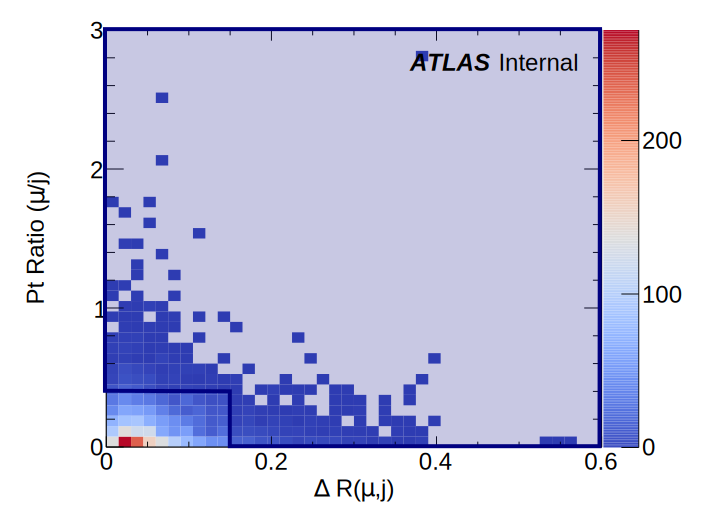
\includegraphics[width=.48\textwidth]{figs/ssww_13tev/custom_or/sig_Muon_DR_PtRatio_edited}
  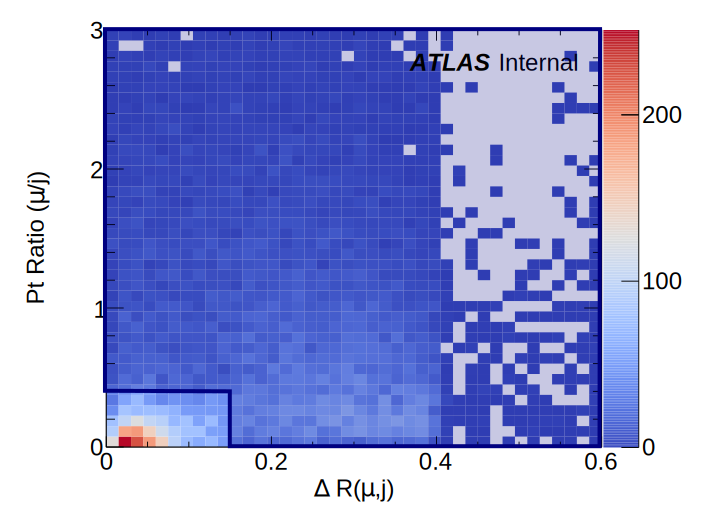
\includegraphics[width=.48\textwidth]{figs/ssww_13tev/custom_or/bkg_Muon_DR_PtRatio_edited}
  \caption{Stuff}
  \label{fig:ssww13tev_customor_muon_2d}
\end{figure}

